%%%%%%%%%%%%%%%%%%%%%%%%%%%%%%%%%%%%%%%%%%%%%%%%%%%%%%%%%%%%%%
%%%%		PLANTILLA LATEX PARA INFORMES
%%%%			LATEX REPORT TEMPLATE
%%%%
%%%%	Autor	: Carlos Gonzalez Cortes
%%%%	Correo	: carlgonz@ug.uchile.cl
%%%%	Version	: 1.0
%%%%
%%%%	Notas	: Este codigo se entrega tal cual es y sin
%%%%			  ningun tipo de garantia. Sientase libre de
%%%%			  modificar y compartir.(acentos omitidos en
%%%%			  los comentarios por compatibilidad)
%%%%
%%%%%%%%%%%%%%%%%%%%%%%%%%%%%%%%%%%%%%%%%%%%%%%%%%%%%%%%%%%%%%




\documentclass[11pt,letterpaper]{article}
\usepackage[spanish]{babel}
%\usepackage[ansinew]{inputenc}
\usepackage[utf8]{inputenc}
% \usepackage[latin1]{inputenc}
\usepackage[letterpaper,includeheadfoot, top=0.5cm, bottom=3.0cm, right=2.0cm, left=2.0cm]{geometry}
\renewcommand{\familydefault}{\sfdefault}

\usepackage{graphicx}
\usepackage{color}
\definecolor{deepblue}{rgb}{0,0,0.5}
\definecolor{deepred}{rgb}{0.6,0,0}
\definecolor{deepgreen}{rgb}{0,0.5,0}
\usepackage{hyperref}
\usepackage{amssymb}
\usepackage{url}
%\usepackage{pdfpages}
\usepackage{fancyhdr}
\usepackage{hyperref}
\usepackage{subfig}
\DeclareFixedFont{\ttb}{T1}{txtt}{bx}{n}{9} % for bold
\DeclareFixedFont{\ttm}{T1}{txtt}{m}{n}{9}  % for normal

\usepackage{listings} %Codigo
\lstset{
language=Python,
basicstyle=\ttm,
otherkeywords={self},             % Add keywords here
keywordstyle=\ttb\color{deepblue},
emph={MyClass,__init__},          % Custom highlighting
emphstyle=\ttb\color{deepred},    % Custom highlighting style
stringstyle=\color{deepgreen},
frame=tb,                         % Any extra options here
showstringspaces=false            %
}

\begin{document}
%\begin{sf}
% --------------- ---------PORTADA --------------------------------------------
\newpage
\pagestyle{fancy}
\fancyhf{}
%-------------------- CABECERA ---------------------
\fancyhead[L]{ 
\includegraphics[scale=0.9]{img/logo.pdf} }
%------------------ TÍTULO -----------------------
\vspace*{6cm}
\begin{center}
\Huge  {Tarea 2}\\
\vspace{1cm}
\huge {Recursive Neural Network}\\
%\vspace{1cm}
%\small {Título pe} \\
\end{center}
%----------------- NOMBRES ------------------------
\vfill
\begin{flushright}
\begin{tabular}{ll}
Autor: & Matías Meneses C.\\
Profesor: & Alex Bergel\\
& \today\\
& Santiago, Chile.
\end{tabular}
\end{flushright}

% ·············· ENCABEZADO - PIE DE PAGINA ············
\newpage
\pagestyle{fancy}
\fancyhf{}

%Encabezado
%\fancyhead[L]{\rightmark}
\fancyhead[L]{\small \rm \textit{Sección \rightmark}} %Izquierda
\fancyhead[R]{\small \rm \textbf{\thepage}} %Derecha


\fancyfoot[L]{\small \rm \textit{Redes Neuronales y Programación Genética}} %Izquierda
\fancyfoot[R]{\small \rm \textit{Tarea 2 - Recursive Neural Network}} %Derecha
%\fancyfoot[C]{\thepage} %Centro

\renewcommand{\sectionmark}[1]{\markright{\thesection.\ #1}}
\renewcommand{\headrulewidth}{0.5pt}
\renewcommand{\footrulewidth}{0.5pt}

% =============== INDICE ===============

\tableofcontents
%\listoffigures

% =============== SECCION ===============
\newpage
\section{Introducción}
El objetivo de esta tarea es realizar una red neuronal avanzada respecto a 
la implementada en la primera tarea del curso.\\

Se decidió realizar una Recursive Neural Network (RNN) que sea capaz de 
generar poemas, entrenándola préviamente con poemas de Pablo Neruda.\\

Se realizaron diversas pruebas para analizar la efectividad de la predicción, 
la sintáxis y semántica del texto generado. Las pruebas fueron realizadas 
variando los parámetros de la red para comprobar su impacto.\\

La inspiración y fuente de información para la implementación fue extraída de estos dos portales 
de internet:

\begin{itemize}
	\item \href{http://karpathy.github.io/2015/05/21/rnn-effectiveness/}{The Unreasonable Effectiveness of Recurrent Neural Networks}
	\item \href{http://www.wildml.com/2015/09/recurrent-neural-networks-tutorial-part-1-introduction-to-rnns/}{Recurrent Neural Networks Tutorial}
\end{itemize}

En este informe se explican brévemente las partes de una RNN.
\subsection{Software utilizado}
Se utilizó el lenguaje de programación Python para realizar la implementación de
la RNN, en conjunto con la librería numpy para realizar el 
cálculo matricial.\\

El programa resultante fue ejecutado en una máquina con Linux (Fedora 26),
intel core i5 con 8 GB de RAM.
\clearpage
\section{Preparación de Input}
Se cuenta con un set de 232 poemas de Pablo Neruda, con un total de $361321$ caracteres. 
El archivo viene con marcadores especiales para separar poemas, estrofas y versos.\\

Se procesa el archivo de tal forma que se genere un vector que contenga todos los versos, 
en formato de vector con el código correspondiente a cada caracter, el cual fue calculado 
previamente.

\begin{figure}[ht!]
\centering 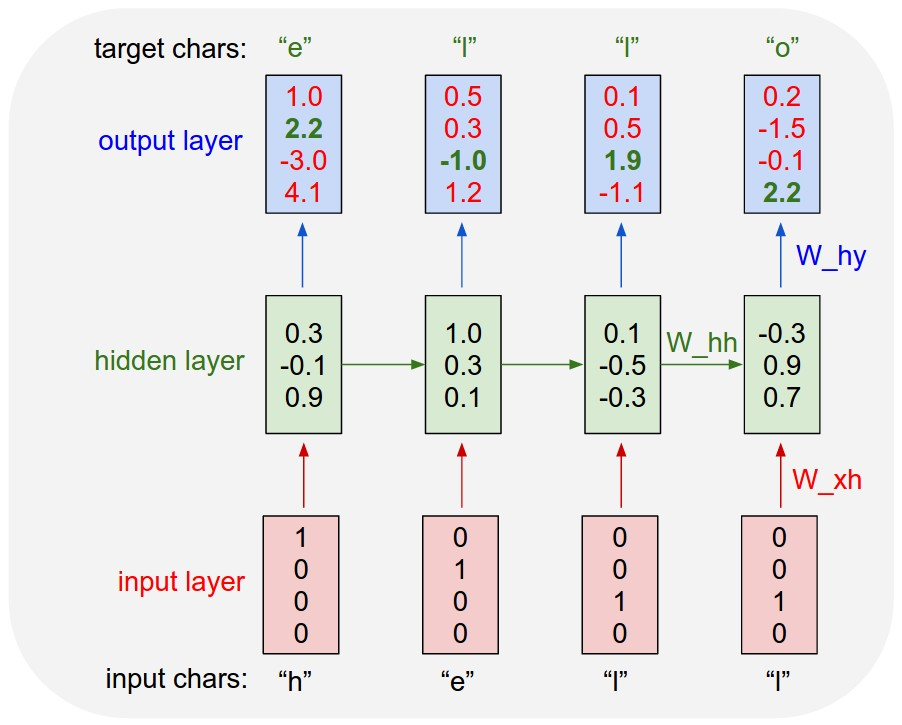
\includegraphics[width=0.5\textwidth]{img/charseq.jpeg}
\caption{Diagrama de la RNN a construir} \label{img1}
\end{figure}

\section{Construcción de Red Neuronal}
A diferencia de la tarea anterior, se usaron matrices para representar las distintas capas 
de la red neuronal, con el objetivo de realizar los algoritmos de forma eficiente realizando 
operaciones sobre matrices. Los siguientes parámetros matriciales caracterizan a la red:

\begin{itemize}
	\item $WXH$: representa los pesos entre el input ($X$) y la capa oculta ($H$)
	\item $WHH$: representa los pesos entre neuronas de la capa oculta. Son la "memoria" de la RNN
	\item $WHY$: representa los pesos entre la capa oculta y el output ($Y$)
	\item $bH$: bias de la capa oculta
	\item $bY$: bias del output
\end{itemize}

Se construyó la red de tal forma que permita cargar estos parámetros desde archivos, con 
el objetivo de realizar sampling posterior, o continuar con el entrenamiento de la red.


\subsection{Forward step}
En este paso, se construyen las representaciones de \textit{hot vector} del input, esto es, 
un array con $1$ en la posición del caracter correspondiente, y $0$ en el resto. Además, 
se realiza el cálculo de los output de las neuronas de la capa oculta y de salida, para 
finalmente calcular el vector distribución de probabilidad final. Para una RNN, las ecuaciones 
son las siguientes:

\begin{itemize}
	\item $h_t = \tanh(WHX \cdot x_t + WHH \cdot h_{t-1} + bH)$
	\item $y_t = WHY \cdot h_t + bY$
	\item $p_t = softmax(y_t)$
\end{itemize}

Se escogió la tangente hiperbólica como función de activación, pues presenta grandientes más fuertes 
que el sigmoid, y tiene un rango mayor. Se utiliza \textit{softmax} para calcular la distribución de probabilidad. $softmax(x) = \frac{\exp x}{\exp {\sum x}}$.

\subsection{Backpropagation}
En este paso se calculan los gradientes de los parámetros de la RNN. Notar que es necesario 
utilizar la derivada de la tangente hiperbólica $\frac{d}{dx}\tanh x = 1 - \tanh^2 x$.

\subsection{Update}
En este paso se actualiza el valor de los parámetros. El error fue calculado en los pasos anteriores 
usando \textit{cross-entropy loss}, y la actualización se realiza usando Adagrad, un tipo de gradiente 
descendiente.

\section{Experimentos}
Se realizaron experimentos con 3 cantidades de epoch distintas. La primera con sólo un epoch, 
la segunda con $200$ epoch y la tercera con $450$ epoch, todas con $100$ capas ocultas y un learning 
rate de $0.1$. Se generó un texto de veinte mil caracteres para todas las configuraciones. Además, para 
la configuración más entrenada, se generó texto realizando variaciones en la decisión probabilística 
del siguiente caracter:

\begin{itemize}
	\item Elección sobre distribución de probabilidad: estándar, usado en la generación de texto
	\item Elegir siempre el caracter con más alta probabilidad
	\item Híbrido entre las dos opciones anteriores: cuando está generando la primera letra de una 
		palabra, usa la distribución de probabilidad, y cuando está generando caracteres 
		dentro de una palabra, usa el caracter con más alta probabilidad
\end{itemize}


\section{Resultados}
\subsection{Sample con 1 epoch}
\begin{center}
\parbox{0.5\linewidth}{
pradarenémir leraco.\\
El sue po,\\
deña\\
ne uatiempa piocisnalcimidóngbren mhjudestojapeque cabre de eliesMeno\\
sebardabarasraas a,\\
lara y emio.\\

Y ernelo erresterloguerer, lo conlotiteudocón\\
s cor ilrarabra mielilo\\
éja cartabre tertrora an os\\
denebrar de quecaba\\
ses ga:\\
havia murtoresinta vera se la? : ve a lontecondo si predron.\\

Y astibontasijos y cunsqumararetetraegodo simar men\\
arlesmia tu
}
\end{center}

\subsection{Sample con 100 epoch}
\begin{center}
\parbox{0.5\linewidth} {
Ascicidon\\
sin mi di los pararás casa,\\
huesta hi atolas sino. Ascos, estávilla.\\

Ahiencia he mi valque verrillos mi arilta paudos ye el agua\\
qué mi vida,\\
al amargamente,\\
como netaza el peso.\\
No tibirmanal, mi mis desiljas orgado\\
que es esosos.\\

Entre emiste el quisando e viocó como impunovas,\\
como pormies!\\
Aho de hetienderes\\
ena bor murés deseralma haja univas no que vieron que árblos, las estura sile segue el otor mara yo mada y entre, que porda, sobre océadas,\\
nadio y este en la vistir, canas en casta, y mi comos en mi vieles entres al anumiras de viento resmbada,\\
es yo sólo de otaúdas y masado dómilelo.\\

Anlos.\\
Amando y modieno\\
encagio, oria!\\
Larnoy manto\\
nos tenó bamo el mi amiqué lejos.\\
Ases y, masta hay me la morvamensiguncarios,\\
como volas que quelundido y del mundos, las hosa.\\
Y\\
pombras y ya, sin altas, ardes que mientos, ciego de Macho!\\
Aques su vida se qué hace y cocinitan se hos que espira pocas como na corre su descia.\\
}
\end{center}

\subsection{Sample con 200 epoch}
\begin{center}
\parbox{0.5\linewidth} {
Nudrisa:\\
el pré andán y dombeso\\
conéjo cuanzante.\\
Cabré tu piema milera,\\
paledas len y escallón que o petán misto\\
mirnendo\\
pascuina de mero interañas enden en el ototeda su talallos vestidos,\\
un umbre las miriderne co pilce al llagamosemos\\
tría que escantas\\
con abitan\\
paraceadorda miempo derdidetrigos:\\
termira brambando caíderte la sigo y no se vejen entrecentimer una picierto az minto rodriempa\\
parabaro así caía!\\
}
\end{center}

\subsection{Samples con 450 epoch}
\subsubsection{Método estándar}
\begin{center}
\parbox{0.5\linewidth} {
Tes que estmpándo,\\
con las aque do,\\
yolmado decico en leño por taste hacio\\
crilles cruel voz el rigredo mía el charas\\
algosoha que el otravas,\\
hastados,\\
con munez\\
y y las hoy de su sanos pájaces\\
este tantirilos,\\
suaroto qué contío viven lego morone?\\

Conturamente me lojas alga, hojas azul mundo,\\
mungaros ola, los nocentia muertes, el alvezas,\\
de un cricales:\\
con los campanados y ar al raíz\\
si por las despetud.\\
}
\end{center}

\subsection{Método de máxima probabilidad}
\begin{center}
\parbox{0.5\linewidth} {
Es el mar en la estrella en la estrella en la estrella en la estrella en la estrella en la estrella ...
}
\end{center}

\subsection{Método híbrido}
\begin{center}
\parbox{0.5\linewidth} {
No sol se sube la luz que me desperas en el tiempo un corazón solo por el hombre las cosas de la que al palente interio de oro de este rosas se para ola de tristeza que la luna con un día a una al palente están gallar o la orrar los piedras algo mi para hora de mi inveridos de humo y el océan la pallas las sembante de despado solo que se la verdidos los piedras por las como para de alviel como bajo estar como invieron jon alegre me para al palente de un las hojas boca la llena de la invia un sus por una un golpera de la una venido a como el hombre con las despado a por como en la recesta en que con alma en la orgulas triste gotalla con despera con alma los alma de palo de la madieron en veces no interan grande las como en la vida en la estrella de la pallas paso un noche la luna en la tierra tu sangre azul por invidado en todo la contigo en la muerte la invierto manos de sueron y ...
}
\end{center}

\section{Análisis de Resultados}
Se observa de los resultados que la sintáxis (estructura) de los poemas fue generada de forma 
satisfactoria, sin haber diferencias significativas respecto a la cantidad de entrenamiento.\\

Con respecto al contenido de los poemas, se observa que mientras más entrenada está la red, 
más palabras correctas logra generar, pero que aún con 450 epoch sigue generando muy pocas 
palabras existentes.\\

Con respecto a la variación en la decisión probabilística, la elección del caracter con más alta 
probabilidad lleva a un loop de usualmente 3 palabras. Estas palabras, sin embargo, son existentes. 
Esta pista fue la que nos llevó a realizar el tercer método híbrido de predicción. Con este método, 
se generaron muchas palabras existentes pero se perdió la estructura de un poema y la puntuación 
del lenguaje. Esto tiene sentido, ya que es más probable que una letra esté acompañada de más letras que de un signo de puntuación o un marcador especial.\\

Los distintos samples pueden ser generados ejecutando los archivos 
\textit{sample\_method.py filename}, y la red puede ser entrenada ejecutando el archivo \textit{train.py}.

\section{Conclusión}
Se concluye que la RNN fue capaz de genera poemas sintácticamente correctos, no así con 
la semántica, generando en su mayoría palabras inexistentes. Se cree que una mayor cantidad de 
entrenamiento, así como un dataset mayor puede generar textos de mayor calidad. Se debe considerar como 
un factor importante que el vocabulario de un poeta es muy amplio.\\

Queda pendiente la realización de otras pruebas con distintos dataset y en inglés, para contrastar los 
resultados considerando el tamaño del vocabulario y las características del idioma. Además, es deseable 
realizar esta implementación utilizando alguna librería de cálculo en GPU como Theano.\\

Como comentario personal, fue una tarea muy entretenida, con la que me hubiera gustado tener más tiempo 
para realizar diversas pruebas, pero eso ya sería más un proyecto semestral que una tarea :) .

% ============= FIN DE DOCUMENTO ==============
\end{document}

% % ················ IMAGEN ·················
% \begin{figure}[ht!]
% \centering
% \fbox{\includegraphics[scale=0.6]{img/flujo.png}}
% \caption{Flujo de caja anual}\label{flujo}
% \end{figure}
% %··········································

% % ················ IMAGEN DOBLE ·················
% \begin{figure}[ht!] \centering
% \subfloat[Esquemático]{\includegraphics[scale=0.44]{img/seguidor.png}}
% \subfloat[Simulación]{\includegraphics[scale=0.45]{img/seguidor1.png}}
% \caption{Simulación como seguidor de voltaje}\label{seguidor}
% \end{figure}
% %··········································
